% -------------------- Premiers pas: ----- 'calculip.tex' --------------------
\section{Premiers pas\ldots}

\markright{Pour bien commencer}

\label{ip}
\subsection{Comment calculer ton adresse IP ?}
%% Calculer l'adresse \emph{IP} de son casert

\label{calcul_ip}

Une adresse IP est une suite de quatre nombres compris entre 0 et
255 s\'epar\'es par des points ; en gros, elle identifie de mani\`ere
unique toute machine connect\'ee au r\'eseau mondial. \emph{Exemple :}
l'adresse IP de \server{frankiz} est \server{129.104.201.51}.

Les adresses IP de l'X sont toutes de la forme \server{129.104.AAA.BBB}.
Les pages suivantes t'indiquent comment calculer \server{AAA} et \server{BBB} pour que ton
ordinateur ait une adresse unique et correcte. Une erreur sur cette adresse t'emp\^eche tout simplement d'acc\'eder au r\'eseau, donc assure-toi que ton calcul est juste !

Calcule ci-dessous ton adresse IP, celle de ta passerelle (\emph{gateway}), ton masque de sous-r\'eseau
(\emph{netmask}) et enfin ton adresse de diffusion (\emph{broadcast}).
Rev\'erifie bien que tu ne t'es pas tromp\'e,  \c{c}a t'\'evitera de te prendre la t\^ete pendant la suite de la configuration !
Note-les soigneusement au bas de la page \pageref{tableauIp} pour référence ultérieure.

\subsubsection{En Maunoury, Foch, Fayolle et Joffre}
Les identifiants \server{AAA} et \server{BBB} se calculent \`a partir de ton num\'ero de casert. \server{BBB} correspond aux deux derniers chiffres. Par exemple, pour le casert $12.10.61$, \server{BBB} $= 61$. \server{AAA} et les autres adresses n\'ecessaires \`a la configuration sont indiqu\'ees dans le tableau ci-dessous, et d\'ependent des quatre premiers chiffres de ton num\'ero de casert, not\'es $xx\ yy$ :
\\
\begin{center}
\begin{tabular}{|>{\ungaramond}c|>{\ungaramond}c|c|c|c|}
\hline \multirow{2}{*}{$xx\ yy$} & \multirow{2}{*}{AAA} & \multirow{2}{*}{\bf Passerelle} & \bf Adresse de  & \bf Masque de  \\ 
 & & & \bf{diffusion} & \bf sous-r\'eseau \\
\hline 09 10 & 220 & \multirow{4}{*}{\server{129.104.223.254}} & \multirow{4}{*}{\server{129.104.223.255}} & \multirow{16}{*}{\server{255.255.252.0}} \\ 
\cline{1-2} 09 20 & 221 &  &  &  \\ 
\cline{1-2} 09 30 & 222 &  &  &  \\ 
\cline{1-2} 09 40 & 223 &  &  &  \\ 
\cline{1-4} 10 10 & 212 & \multirow{4}{*}{\server{129.104.215.254}} & \multirow{4}{*}{\server{129.104.215.255}} & \\ 
\cline{1-2} 10 20 & 213 &  &  &  \\ 
\cline{1-2} 10 30 & 214 &  &  &  \\ 
\cline{1-2} 10 40 & 215 &  &  &  \\ 
\cline{1-4} 11 10 & 232 & \multirow{4}{*}{\server{129.104.235.254}} & \multirow{4}{*}{\server{129.104.235.255}} & \\ 
\cline{1-2} 11 20 & 233 &  &  &  \\ 
\cline{1-2} 11 30 & 234 &  &  &  \\ 
\cline{1-2} 11 40 & 235 &  &  &  \\ 
\cline{1-4} 12 10 & 216 & \multirow{4}{*}{\server{129.104.219.254}} & \multirow{4}{*}{\server{129.104.219.255}} & \\ 
\cline{1-2} 12 20 & 217 &  &  &  \\ 
\cline{1-2} 12 30 & 218 &  &  &  \\ 
\cline{1-2} 12 40 & 219 &  &  &  \\ 
\hline
\end{tabular} 
\end{center}

\exemple{l'adresse IP associ\'ee au casert $12.10.61$ est \server{129.104.216.61}, sa passerelle est \server{129.104.219.254}, son adresse de
diffusion est \server{129.104.219.255} et son masque de sous-r\'eseau est \server{255.255.252.0}.}

\subsubsection{Résidences Schaeffer et Lemonnier}

Ta prise r\'eseau poss\`ede un num\'ero \`a 6 chiffres de la forme $xx\ yy\ zz$. On prend $xx$ pour calculer ton sous-r\'eseau, l'adresse de ta passerelle (\emph{gateway}): \server{129.104.AAA.CCC} et l'adresse de diffusion (\emph{broadcast}): \server{129.104.AAA.EEE}. Le masque de sous-r\'eseau (\emph{netmask}) est toujours
\server{255.255.255.128}. Ensuite, tu peux d\'eterminer la partie \server{BBB} de ton IP avec $zz$ et $xx$ :


\begin{center}
\begin{tabular}{|>{\ungaramond}c|>{\ungaramond}c|>{\ungaramond}c|>{\ungaramond}c|>{\ungaramond}c|}
\hline \rule[-2ex]{0pt}{5ex}$xx$ & $AAA$ & $CCC$ & $EEE$ & $BBB$\\ 
\hline 70 & 224 & 254 & 255 & $128+zz$ \\
71 & 224 & 126 & 127 & $zz$ \\
72 & 228 & 254 & 255 & $128+zz$ \\
73 & 225 & 126 & 127 & $zz$ \\
74 & 225 & 254 & 255 & $128+zz$ \\
75 & 226 & 126 & 127 & $zz$ \\
76 & 227 & 126 & 127 & $zz$ \\
77 & 227 & 254 & 255 & $128+zz$ \\
78 & 228 & 126 & 127 & $zz$ \\
79 & 229 & 126 & 127 & $zz$ \\
80 & 226 & 254 & 255 & $128+zz$ \\ \hline
\end{tabular} 
\end{center}

\exemple{l'adresse IP associ\'ee \`a la prise $70 30 30$ est \server{129.104.224.158} ($158 = 128 + 30$) ; sa passerelle est \server{129.104.224.254}, son
adresse de diffusion est \server{129.104.224.255} et son masque de sous-r\'eseau est \server{255.255.255.128}.}

\subsubsection{Au BEM}

\newlength{\ecart}
\settowidth{\ecart}{Masque de sous-reseau}
\addtolength{\ecart}{2em}
\noindent \begin{tabular}{p{\ecart}<{\dotfill}@{}l}
  Sous-r\'eseau (\server{AAA}) & {\ungaramond 203} pour le bâtiment A ; {\ungaramond 204} pour le bâtiment D\\
  IP (\server{BBB})            & {\ungaramond 50} + les deux derniers chiffres du num\'ero de ta chambre \\
  Passerelle                   & \server{129.104.AAA.13} \\
  Masque de sous-r\'eseau     & \server{255.255.255.0} \\
    Adresse de diffusion       & \server{129.104.AAA.255} \\
\end{tabular}

\subsubsection{Au PEM}

 \noindent \begin{tabular}{p{\ecart}<{\dotfill}@{}l}
  Sous-r\'eseau (\server{AAA})           & {\ungaramond 205} \\
  IP (\server{BBB}), rez-de-chauss\'ee & {\ungaramond 15} + les deux derniers chiffres du num\'ero  de ta chambre \\
  IP (\server{BBB}), premier \'etage   & {\ungaramond 70} + les deux derniers chiffres du num\'ero de ta chambre \\
  Passerelle                             & \server{129.104.205.13} \\
  Masque de sous-r\'eseau                & \server{255.255.255.0} \\
  Adresse de diffusion                   & \server{129.104.205.255} \\
\end{tabular}

% \subsubsection{IP des serveurs DNS}
%
% Le BR offre quatre serveurs DNS redondants, qui ont les IP's suivantes :
% \begin{itemize}
%   \item Serveur principal : $129.104.201.53$
%   \item Serveurs secondaires : $129.104.201.51$, $129.104.201.52$ et $129.104.201.54$
% \end{itemize}

\pagebreak


% -------------------- Les differentes configs --------------------

\markright{Configuration sous Windows}
\label{windows}
\bghdr{images/fond-win}

%\begin{center}
%
\includegraphics{images/logo_Windows}
%\end{center}


\subsection{Configuration sous Microsoft Windows}

%Cette section décrit comment configurer un ordinateur tournant sous Windows XP, Windows Vista, Windows 7 ou Windows 8. Si tu possèdes une autre version de Windows,
%nous t'invitons à  regarder directement la section sur les licences MSDNAA en page \pageref{msdnaa}\dots ou alors à  te débrouiller ! ;-)
%
%\subsubsection{Configuration IP}
%
%\begin{itemize}
%
%\item \textbf{Sous Windows XP :} va dans le \menu{Menu Démarrer}, \menu{Panneau de configuration} et double-clique sur \menu{Connexions réseau} puis sur \menu{Connexion au réseau local}. Clique enfin sur \menu{Propriétés}.
%
%\item \textbf{Sous Windows Vista :} va dans le \menu{Menu Démarrer}, \menu{Panneau de configuration}, \menu{Réseau et Internet}, \menu{Centre réseau et partage}. Là, dans le menu à  gauche, clique sur \menu{Gérer les connexions réseau}, puis clique droit sur \menu{Connexion au réseau local} et enfin  \menu{Propriétés}~\footnote{ÀA ce stade, ainsi qu'à  plusieurs autres étapes de ce tutoriel, Windows Vista doit normalement t'afficher un message te demandant de confirmer l'action que tu viens d'effectuer. Donc tu confirmes, et cela à  chaque fois !}.
%
%\item \textbf{Sous Windows 7 et Windows 8 :} va dans le \menu{Menu Démarrer} (Windows 7) ou le \menu{Menu Paramètres} (Windows 8), \menu{Panneau de configuration}, \menu{Réseau et Internet}, \menu{Centre réseau et partage}, \menu{Modifier les paramètres de la carte}. Puis clique droit sur \menu{Connexion au réseau local} et enfin  \menu{Propriétés}.
%
%\end{itemize}
%
%
%
%%\flimage{images/win_connexion_icone}{0.15}{l} Va dans le \menu{Menu
%%Démarrer}, \menu{Panneau de configuration} et double-clique sur
%%\menu{Connexions réseau} puis sur \menu{Connexion au réseau local}.
%%Clique enfin sur \menu{Propriétés}.\\
%
%%Dans cette fenêtre, coche les trois cases \menu{Client pour les
%%réseaux Microsoft}, \menu{Partage de fichiers} et \menu{Protocole
%%Internet (TCP/IP)}:
%
%\imagepos{images/win_config_connexion2}{0.5}{Configurer la connexion au réseau local}{!h}
%
%
%
%%\imageref{images/win_config_ip}{0.5}{Configuration IP --- Propriétés de protocole Internet (TCP/IP)}{!ht}{config:win:IP1}
%%%%%\imageref{images/win_config_ip2}{0.71}{Configuration de la connexion
%%au réseau local et propriétés du TCP/IP}{!ht}{config:win:IP1}
%
%Sélectionne ensuite la ligne \menu{Protocole Internet Version 4 (TCP/IPv4)}~\footnote{\menu{Protocole Internet (TCP/IP)} pour certaines versions de Windows XP.},
%puis clique sur le bouton \menu{Propriétés} qui vient de se
%dégriser. Tu tombes alors sur l'écran de configuration de ta
%connexion vers l'extérieur.
%
%\noindent
%  \begin{figure*}[!h]
%    \begin{center}  
%      \subfloat[Configuration IP --- Propriétés de protocole Internet (TCP/IP)]{ 
%      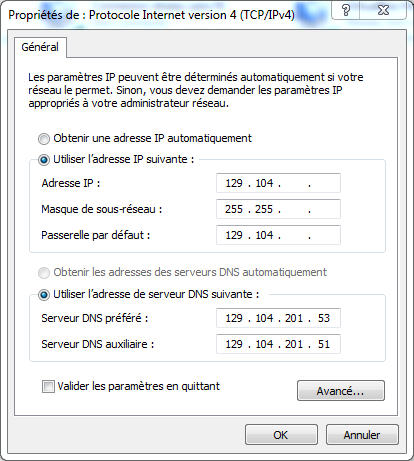
\includegraphics[width=0.48\textwidth]{images/win_config_ip} \label{config:win:IP1}}
%      \hspace{\stretch{1}}
%      \subfloat[Configuration DNS]{ 
%         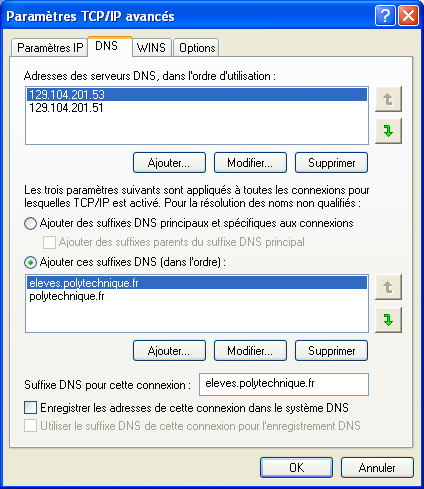
\includegraphics[width=0.48 \textwidth]{images/win_config_dns2} \label{config:win:IP2}}
%             \caption{Configuration réseau}
%    \end{center}
%  \end{figure*}
%
%
%
%%% \newpage
%Coche alors les cases \menu{Utiliser l'adresse IP suivante} et \menu{Utiliser l'adresse de serveur DNS suivante} et remplis les cinq champs d'adresse IP. Tu trouveras toutes les valeurs d'adresse IP nécessaires pour la configuration en page~\pageref{tableau:mon_IP} ; aide-toi de la capture d'écran~\ref{config:win:IP1} pour les placer. Si une partie d'adresse IP est blanche sur cette capture, c'est qu'elle t'est personnelle et que tu dois la calculer !
%Clique ensuite sur le bouton \menu{Avancé}, puis sur l'onglet
%\menu{DNS} en haut.
%Il n'y a plus qu'à  remplir les différents champs comme sur la
%capture d'écran suivante, avec le bouton \menu{Ajouter} et les
%flèches pour réordonner les éléments.
%
%
%%\subsubsection{Le domaine Windows}
%
%%\paragraph{Qu'est ce que c'est ?}
%%Le domaine Windows est un système d'automatisation de la
%%configuration de plusieurs ordinateurs sous Windows situés sur le
%%même réseau. En fait, c'est un outil d'administration, conçu par
%%exemple pour des entreprises où un service informatique doit gérer
%%de nombreuses machines; il permet d'appliquer des modifications de
%%configuration à  toutes les machines du domaine directement depuis un
%%serveur. Le BR possède un serveur dédié au domaine Windows,
%%\server{enez}.
%
%%Le domaine met à  jour automatiquement Windows et l'antivirus à  partir d'\server{enez} (très rapide car tu n'as pas besoin de récupérer des fichiers
%%en dehors de l'école!). Il configure le \emph{firewall} (pare-feu: système de protection contre les éventuelles attaques par le réseau) Windows, mais
%%il est toujours possible de le désactiver si tu préfères un autre \emph{firewall}. En bref, il permet de simplifier à  l'extrême %la mise à  jour
%%continuelle de l'ordinateur.%
%
%
%%\paragraph{Alors, domaine ou pas domaine ?} Soit tu choisis de te
%%mettre sur le domaine Windows, et tu vas alors au paragraphe
%%\guillemotleft~Inscription sur le domaine Windows~\guillemotright.%
%
%%% \newpage
%%\textbf{Avantages :}
%%\begin{itemize}
%%\item Windows est mis à  jour automatiquement ; tu as toujours les
%%dernières corrections de sécurité et un pare-feu correctement
%%configuré. Donc tu es mieux protégé contre les intrusions.
%%\item Surtout, tu n'as plus à  t'en occuper, presque tout est automatique.
%%\end{itemize}%
%
%%\textbf{Inconvénients :}
%%\begin{itemize}
%%  \item Tu délègues une partie des droits d'administration de ta machine au BR
%%        (tout ce qui concerne la sécurité du réseau en particulier).
%%        Cependant, si tu ne sais pas le faire, c'est plutôt un avantage
%%        de laisser le BR s'en occuper à  ta place.
%%  \item Cela ne marche qu'avec Windows 2000, Windows XP Pro ou Windows Vista Business.
%%        On te rappelle que tu peux facilement, gratuitement et légalement passer à 
%%        Windows XP Pro ou bien à  Windows Vista Business (section sur les licences
%%        MSDNAA en page \pageref{msdnaa}).
%%\end{itemize}
%
%%Bien s\^{u}r, tu peux sortir du domaine à  tout instant, et effectuer manuellement les réglages nécessaires à  la sécurité de ton ordinateur.
%
%%Soit tu choisis de configurer toi-même ton ordinateur, et tu peux passer
%%directement à  la section \guillemotleft Installation de l'antivirus
%%\guillemotright. Tu trouveras les informations nécessaires à  la configuration
%%manuelle du pare-feu et du proxy pour \app{Windows Update} en annexe à  la
%%fin de cette section, en page \pageref{horsdomaine}.
%
%%\textbf{Avantage :} Tu es le seul à  t'occuper de la gestion de ton ordinateur.
%
%%\textbf{Inconvénient :} Tu es le seul à  t'occuper de la gestion de ton ordinateur. ;-)
%%S'il devient un foyer pour virus, sache que nous avons les moyens de l'isoler
%%pour éviter toute propagation.
%
%%\begin{center}
%%  \fbox{
%%    \begin{minipage}{.7\textwidth}
%%      \begin{center}
%%Le BR te conseille \emph{très fortement} de te mettre sur le domaine
%%et de choisir l'installation simplifiée !
%%      \end{center}
%%    \end{minipage}
%%  }
%%\end{center}
%
%
%%\paragraph{Inscription sur le domaine Windows}
%
%%On te rappelle que tu ne peux t'inscrire sur le domaine que si tu utilise
%%Windows 2000, Windows XP Pro ou Windows Vista. Si tu possède Windows XP
%%Familial, Windows Vista Home ou encore une version antérieure de Windows,
%%tu dois effectuer toi-même tes réglages de pare-feu et de proxy
%%\app{Windows Update}. Réfère-toi pour cela à  l'annexe ad hoc à  la fin de
%%cette section, en page \pageref{horsdomaine}.
%
%%La procédure d'inscription est la suivante :
%%\begin{itemize}
%
%%\item \textbf{Sous Windows XP :} Clique sur le \menu{Menu Démarrer} puis fais un clic-droit sur
%%\menu{Poste de travail} et choisis \menu{Propriétés}. Ensuite, sélectionne l'onglet \menu{Nom de l'ordinateur} et clique le bouton \menu{Modifier}.
%
%%\item \textbf{Sous Windows Vista :} Clique sur \menu{Menu Démarrer}, puis fais un clic-droit sur \menu{Ordinateur}, \menu{Propriétés}. Là  sélectionne \menu{Paramètres système avancés}, onglet \menu{Nom de l'ordinateur}, puis clique sur le bouton \menu{Modifier}.
%
%%\end{itemize}
%
%%Dans la case \menu{Nom de l'ordinateur}, rentre ton pseudo, puis coche la case \menu{domaine} et
%%rentre \urllink{windows.eleves.polytechnique.fr}. Note bien que l'inscription au domaine te sera
%%refusée par le serveur si quelqu'un d'autre utilise déjà  le même nom d'ordinateur que toi. Par
%%conséquent, essaie d'opter pour un pseudo qui t'identifie de façon claire et unique, par exemple
%%\cmd{NOM\_PRENOM} \footnote{Les Jean Dupont et les Julien Thomas sont priés de trouver autre chose
%%;-)}.
%
%%\imagepos{images/win_config_domaine}{0.5}{S'inscrire sur le domaine windows}{!ht}
%
%%\begin{center}
%%\begin{tabular}{ll}
%% \parbox{.45\textwidth}{
%%  et si tu es rouje 2006 :
%%  \begin{description}
%%    \item[Nom] rouje06
%%    \item[Mot de passe] rouje.2006
%%  \end{description}
% % }
%% & \parbox{.45\textwidth}{
%%  Si tu es jône 2007, tu rentres :
%%  \begin{description}
%%    \item[Nom] jone07
%%    \item[Mot de passe] jone.2007
%%  \end{description}
%%  }
%%\\
%%\end{tabular}
%%\end{center}
%
%%\emph{Attention, ces identifiants servent juste à  t'inscrire sur le
%%domaine. Pour utiliser ton ordinateur, tu devras rentrer au
%%démarrage les mêmes nom d'utilisateur et mot de passe que tu avais
%%avant d'être sur le domaine !}
%%
%%
%%
%%%\paragraph{Installation personnalisée} --- configuration manuelle
%
%%\subparagraph{Configuration antivirus} Le BR, concerné par la
%%sécurité du réseau, te propose un antivirus pour lequel tu n'auras
%%pas à  payer la license pour obtenir les mises à  jour. Bien sà�¿½r,
%%libre à  toi d'utiliser ton anti-virus personnel ; cependant il sera
%%à  ta charge de le mettre à  jour très réguliérement. Pour cela
%%utilise comme proxy : \urllink{http://kuzh} sur le port 8080.
%
%%\emph{Installation de l'anti-virus du BR}\ : Commence par
%%désinstaller tous les antivirus ou firewalls que tu pourrais avoir
%%comme expliqué dans le paragraphe \guillemotleft~Installation simplifiée
%%--- configuration automatique~\guillemotright .
%
%%Puis ouvre ton explorateur Windows et tape :
%%\urllink{$\backslash\backslash$enez$\backslash$antivirus}
%%et double-clique sur le fichier \file{Symantec.exe}.
%
%%Ce package contient le paramétrage de la mise à  jour automatique de
%%Windows sur le serveur de l'école. Attends la fin de l'installation
%%et c'est fini ! Maintenant, tu n'as plus à  toucher à  l'antivirus,
%%normalement il sera mis à  jour automatiquement.
%
%%\subparagraph{Configuration firewall}
%
%%Si tu as Windows XP avec le SP2 installé, tu as un firewall
%%automatiquement activé et facile d'utilisation. En effet, à  chaque
%%fois qu'un programme tentera d'aller pour la première fois sur
%%Internet, il te demandera si tu veux le laisser faire ou non, comme
%%dans la capture~\ref{config:win:firewall}.
%
%%\imageref{images/win_firewall}{0.8}{Un programmme --- ici GuildFTP
%%--- demande à  accéder au réseau}{!ht}{config:win:firewall}
%
%%Le firewall commercial \app{ZoneAlarm}, indépendant de Windows,
%%fonctionne sur le même principe. Tu peux le trouver sur \xshare.
%
%%Si tu préfères utiliser le firewall intégré à  Windows XP (sans le
%%SP2) ou à  Windows Server 2003, il te faudra le configurer en détail.
%%Va dans le \menu{Menu Démarrer}, \menu{Paramètres} et clique sur
%%\menu{Connexions Réseau}. Choisis la connexion qui est utilisée par
%%ton ordinateur (souvent il n'y en a qu'une, ou alors une seule est
%%activée) et double-clique dessus. Clique sur \menu{Propriétés} en
%%bas à  gauche, puis sur l'onglet \menu{Avancé} et rentre dans le menu
%%de \menu{Paramètres} du \menu{Pare-feu Windows}. Il te faudra alors
%%ajouter manuellement tous les ports que tu veux ouvrir sur
%%l'extérieur. Pour cela, clique sur \menu{Ajouter}, et remplis la
%%boà�¿½te de dialogue en t'aidant de la capture
%%d'écran~\ref{config:win:ouvrir_port}; mets le numéro du port que tu
%%veux ouvrir, par exemple 5050, 5053 et 5055 en TCP pour \app{qRezix}
%%et 21 en TCP pour ton FTP.
%
%%\imageref{images/win_config_firewall}{0.7}{Ouvrir un port dans le firewall %Windows}{!ht}{config:win:ouvrir_port}
%
%%Comme tu peux le constater, il est beaucoup plus pratique d'aller
%%sur le domaine et de laisser le SP2 faire le gros du boulot à  ta
%%place :-).
%
%
%
%\subsubsection{Configuration \emph{web} (serveur mandataire)}
%
%\imageref{images/win_config_proxy}{0.5}{Configuration du serveur mandataire (\emph{proxy})}{!ht}{config:win:proxy}
%
%Même si tu n'utilises pas \app{Internet Explorer} comme client \emph{web}, Windows et d'autres programmes
%utilisent ses paramètres, notamment \app{Windows Update}. Par conséquent lance \app{Internet Explorer} et va
%dans le menu \menu{Outils}, \menu{Options Internet}, puis sur l'onglet \menu{Connexions} de la
%nouvelle fenêtre et enfin sur \menu{Paramètres réseau} dans le bas de la fenêtre. Tu dois être arrivé sur une fenêtre semblable à celle de la capture d'écran~\ref{config:win:proxy}. Là, coche
%uniquement la case \menu{Utiliser un script de configuration automatique}, puis remplis le champ
%\menu{Adresse} avec \urllink{http://config/proxy.pac}.
%
%Une fois que tu as fait ça, tu n'as plus forcément besoin d'\app{Internet Explorer}, tu peux donc utiliser un autre navigateur, comme \app{Mozilla
%Firefox}, disponible sur \urllink{http://www.mozilla-europe.org/fr/products/}.
%
%Même si tu ne configures pas Windows Update avec le paragraphe ci-dessous, n'oublie pas de régler ton navigateur \emph{web} et ton client \emph{mail} si tu en as un : reporte-toi page \pageref{browser}.
%
%\subsubsection{Windows Update}
%
%\label{horsdomaine} %\emph{Cette sous-section ne concerne pas les gens qui ont choisi de s'inscrire sur le domaine.}
%
%%\paragraph{Pare-feu} Si tu as Windows XP avec le SP2 installé, ou \emph{a fortiori}
%%Windows Vista, tu as un \emph{firewall} automatiquement activé et facile d'utilisation. En effet, à  chaque fois qu'un programme tentera d'aller pour
%%la première fois sur Internet, il te demandera si tu veux le laisser faire ou non. Si tu préfères une protection indépendante de Windows, le
%%\emph{firewall} commercial \app{Zone\-Alarm} fonctionne sur le même principe. Tu peux le trouver sur \xshare.
%
%%Si tu préfères utiliser le \emph{firewall} intégré à  Windows XP (sans le SP2), il te faudra le configurer en détail. Va dans le \menu{Menu Démarrer},
%%\menu{Paramètres} et clique sur \menu{Connexions Réseau}. Choisis la connexion qui est utilisée par ton ordinateur (souvent il n'y en a qu'une, ou
%%alors une seule est activée) et double-clique dessus. Clique sur \menu{Propriétés} en bas à  gauche, puis sur l'onglet \menu{Avancé} et rentre dans le
%%menu de \menu{Paramètres} du \menu{Pare-feu Windows}. Il te faudra alors ajouter manuellement tous les ports que tu veux ouvrir sur l'extérieur. Pour
%%cela, clique sur \menu{Ajouter}, et remplis la boîte de dialogue% en t'aidant de la capture d'écran~\ref{config:win:ouvrir_port} ci après
%%; mets le numéro du port que tu veux ouvrir, par exemple 5050, 5053 et 5055 en TCP pour \app{qRezix} et 21 en TCP pour ton FTP.
%
%Il reste une dernière configuration de
%serveur mandatataire indispensable pour que puissent se faire les mises à  jour automatiques
%de Windows. Il t'est fortement recommandé de le faire.
%
%\begin{description}
%
%\item[Sous Windows 7 \& Windows 8] Si tu as correctement configuré ton serveur \emph{web} mandataire, les mises à jours se font automatiquement.
%
%\item[Sous Windows XP] Fais \menu{Démarrer}, \menu{Exécuter}, puis
%tape \cmd{cmd} dans la fenêtre qui s'affiche. Une ligne de commande apparaît,
%il te suffit alors de taper : \cmd{proxycfg -p http://kuzh:8080} pour régler
%le serveur mandataire. Pour revenir à  un accès direct il faut taper \cmd{proxycfg -d}.
%
%\item[Sous Windows Vista]
%Dans le menu \menu{Démarrer}, tape \guillemotleft~Invite de commandes~\guillemotright{} dans le champ \menu{Rechercher}, puis clique droit sur le lien
%et choisis \menu{Exécuter en tant qu'administrateur}. Tape ensuite les commandes suivantes :
%\cmdline{
%C:\textbackslash{}Windows\textbackslash{}system32$>$netsh\\
%netsh>winhttp\\
%netsh winhttp>set proxy proxy-server="http://kuzh:8080"\\
%netsh winhttp>exit\\
%C:\textbackslash{}Windows\textbackslash{}system32>exit }
%
%Pour revenir à l'accès direct, il suffit de taper :
%\cmdline{
%  netsh winhttp reset proxy
%}
%
%Pour la suite de ta configuration, rendez-vous page \pageref{browser} pour faire marcher ton navigateur web préféré !
%
%\end{description}

%\clearpage


\markright{Configuration sous Linux}
\label{ubuntu}
%$Id: config_nux.tex 145 2005-03-25 08:26:35Z myk $

\bghdr{images/fond_ubuntu}



%\begin{center}
%
\includegraphics{images/logo_Linux}
%\end{center}

\subsection{Configuration sous Ubuntu/Kubuntu}

Cette section décrit la configuration de ta connexion Internet sous Ubuntu GNU/Linux (ou une de ses variantes). Pour les autres distributions, tu peux adapter les instructions ci-dessous ou consulter la version 
en ligne de commande, page \pageref{linux_cmdline}.

\subsubsection{Configuration IP}
Tu as besoin de conna\^itre ton adresse IP, ton masque de sous-r\'eseau et ta  passerelle. Toutes les informations se trouvent page \pageref{calcul_ip}. Bien s\^ur, pour  l'ensemble des manipulations d\'ecrites ci-dessous tu auras besoin de ton  mot de passe super-utilisateur (\emph{root}) !

\label{Ubuntu:IP}
Il existe deux mani\`eres de configurer tes param\`etres r\'eseaux: l'une utilise les outils graphiques de l'environnement que tu as choisi (Gnome ou KDE), 
l'autre utilise simplement la ligne de commande. Bien sûr, les outils graphiques ne sont qu'un interm\'ediaire modifiant les fichiers dont on te parle 
plus bas. Ils te permettent parfois d'enregistrer une configuration r\'eseau, ce qui facilite la gestion si tu rentres souvent chez toi. Pour obtenir le 
m\^eme r\'esultat en ligne de commande il faut utiliser un script.
\begin{description}
\item[\'Etape 1 : configuration de la connexion au r\'eseau] \
 
\begin{itemize}
\item Va dans \menu{Syst\`eme}, \menu{Pr\'ef\'erences} puis \menu{Connexions r\'eseau}.
\item Dans l'onglet \menu{Filaire}, clique sur \menu{Ajouter}.
\item Compl\`ete le champ \menu{Nom de la connexion}  par ce que tu veux ; "Casert de Polytechnique" par exemple.
\item Puis va dans l'onglet \menu{Param\`etres IPv4}.
\item S\'electionne la m\'ethode \menu{Manuel}.
\item Clique sur \menu{Ajouter}, puis remplis les champs \menu{Adresse}, \menu{Masque de r\'eseau} et  \menu{Passerelle} par les donn\'ees qui te sont propres. 
\item Compl\`ete le  champ \menu{Serveurs DNS} par \server{129.104.201.53, 129.104.201.51} et le champ \menu{Domaines de recherche} par \server{eleves.polytechnique.fr, polytechnique.fr}. 
\item Coche enfin l'option \menu{Disponible pour tous les utilisateurs}, clique sur \menu{Appliquer} et enfin rentre ton mot de passe super-utilisateur (root).
\end{itemize}

\item[\'Etape 2 : configuration du proxy (= serveur mandataire)] \
\begin{itemize}
\item Va  dans \menu{Param\`etres Syst\`eme}, \menu{R\'eseau} puis \menu{Serveur Mandataire}.
\item S\'electionne  la \menu{M\'ethode} \menu{Automatique}.
\item Compl\`ete le champ  \menu{URL de configuration} par \urllink{http://config/proxy.pac}. 
\item Clique sur \menu{Appliquer à tout le syst\`eme...} et rentre ton mot de passe super-utilisateur si on te le demande.
\end{itemize}

\item[\'Etape 3 (\'eventuellement)] \
\begin{itemize}
\item Clique  sur l'ic\^one de l'applet R\'eseau dans la zone de notification, en forme  de fl\`eches t\^ete-b\^eche ou d'ondes. S\'electionne le r\'eseau que tu as  configur\'e dans la 1\`ere \'etape, et te voilà connect\'e à Internet !
\item Une fois ta configuration r\'eseau termin\'ee, tu peux la tester en \emph{pinguant} \fkz (dans une console), o\`u tu devrais voir quelque chose comme :
\end{itemize}

\cmdline{\$ ping frankiz\\
PING frankiz.eleves.polytechnique.fr (129.104.201.51) 56(84) bytes of data.\\
64 bytes from Frankiz.eleves.polytechnique.fr ...}

\end{description}



\subsubsection{Configuration du gestionnaire de paquets}
\label{ubuntu_mirror}

Il faut d\'esormais configurer le gestionnaire de paquets pour qu'il utilise les miroirs du BR et non les miroirs à l'ext\'erieur du campus, qui sont plus lents. \
Va  dans \menu{Applications}, \menu{Logith\`eque Ubuntu} puis menu \menu{\'edition}, \menu{Sources de logiciels...}. 
Entre ton  mot de passe super-utilisateur puis s\'electionne l'onglet \menu{Autres  logiciels}. 
D\'ecoche les cases comprenant une adresse du type \urllink{http://archive.canonical.com/ubuntu version}, o\`u \textit{version} correspond à la version d'Ubuntu install\'ee sur ton ordinateur. 
À l'impression de l'InfoBR, la version actuelle est \textbf{oneiric} et la pr\'ec\'edente est \textbf{natty}. \
Clique sur \menu{Ajouter}, puis entre dans le champ \menu{Ligne APT} :
\cmdline{deb ftp://miroir/linux/ubuntu version main restricted universe multiverse}
Tu auras bien s\^ur remplac\'e \textit{version} par ta version d'Ubuntu (\textit{maverick}/\textit{lucid}/\textit{karmic}/...). \\
Clique ensuite sur \menu{Ajouter une source de mise à jour}. Fais de même pour les lignes suivantes :
\cmdline{deb ftp://miroir/linux/ubuntu version-updates main restricted universe  multiverse \\
deb ftp://miroir/linux/ubuntu version-security main restricted universe  multiverse}
Tu peux aussi utiliser le d\'ep\^ot suivant mais attention il contient des logiciels non support\'es par Canonical, l'\'equipe de d\'eveloppement d'Ubuntu (en particulier il peut arriver que certains logiciels contiennent des erreurs) :
\cmdline{deb ftp://miroir/linux/ubuntu version-backports main restricted universe multiverse}
Le  BLL (Binet Logiciels Libres) dispose par ailleurs d'un miroir  non-officiel qui contient des paquets (flash, ...) non  inclus dans la distribution de base pour diverses raisons, en paticulier l\'egales ou \'ethiques. Pour en profiter, rajoute aussi la ligne :
\cmdline{deb ftp://miroir/linux/bll version main}
Clique enfin sur \menu{Fermer} puis r\'eponds \menu{Actualiser} à la fenêtre de dialogue qui appara\^it. \\

Note : il n'est pas n\'ecessaire de configurer Synaptic dans ses Pr\'ef\'erences pour y sp\'ecifier un proxy quelconque.

\subsubsection{Configuration antivirus}

{C'est pas non plus comme si y'en avait besoin \dots}

%\subsubsection{Configuration du pare-feu}
%
%La solution la plus simple pour se faire un \emph{firewall} sous linux est d'utiliser les \emph{iptables}. Pour ceci la premi\`ere \'etape est
%d'installer le paquet \app{iptables} pour ta distribution. Pour savoir comment configurer ton \emph{firewall} pour le r\'eseau de l'X, consulte le Wikix.

\clearpage


\markright{Configuration sous Mac OS}
\label{mac}
\bghdr{images/fond-mac}

%\begin{center}
%
\includegraphics{images/logo_Mac}
%\end{center}



\subsection{Configuration sous Mac OS X}

La configuration est d\'etaill\'ee pour Mac OS 10.5 (\app{Leopard}). %et encore un peu pour Mac OS 10.4 (Tiger).
Afin de conna\^itre la version que tu utilises, va dans le \menu{menu Pomme} puis s\'electionne \menu{\`A propos de ce Mac}.

\subsubsection{Configuration IP}

\flimage{images/mac_prefs_icone}{0.07}{l}
 \app{Pr\'ef\'erences R\'eseau}, accessible depuis l'article de menu \menu{Pr\'ef\'erences syst\`eme} du menu \menu{Pomme}, permet de configurer la connexion au r\'eseau. Par ailleurs, si au d\'emarrage un assistant te propose de configurer ton r\'eseau, refuse et utilise la proc\'edure du BR. En effet, le r\'eseau n\'ecessite une configuration particuli\`ere  \`a l'X, plus complexe que celle effectu\'ee par cet assistant.


\noindent
  \begin{figure*}[h]
    \begin{center}  
     % \subfloat[Tiger]{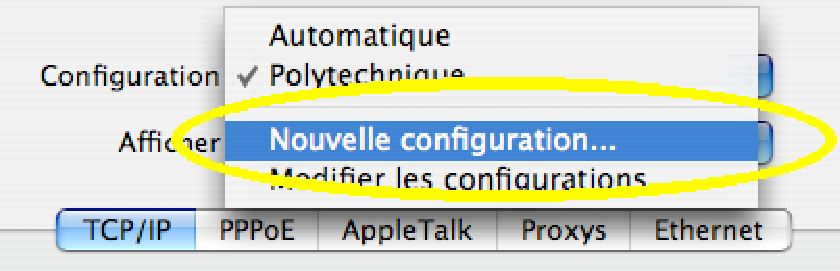
\includegraphics[width=0.47\textwidth]{images/mac_nouvelle_config} } 
     % \hfill
      \subfloat[Cr\'eer une nouvelle configuration r\'eseau]{ 
      \begin{minipage}{0.43 \textwidth}\begin{flushleft}
      {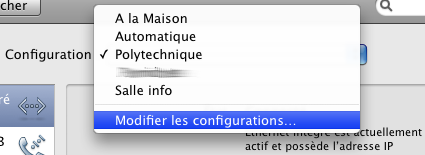
\includegraphics[width=0.96\textwidth]{images/mac_nouvelle_config_leopard_1}}\\ \vspace*{2cm}
      {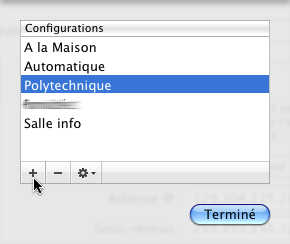
\includegraphics[width=0.96\textwidth]{images/mac_nouvelle_config_leopard_2}} 
 		\end{flushleft}  \end{minipage}
 		 } 		
 		\subfloat[Configuration de l'interface r\'eseau \emph{Ethernet}, de l'adresse IP et du \emph{proxy}]{ 
 		 \begin{minipage}{0.43 \textwidth}\begin{flushright}
 		{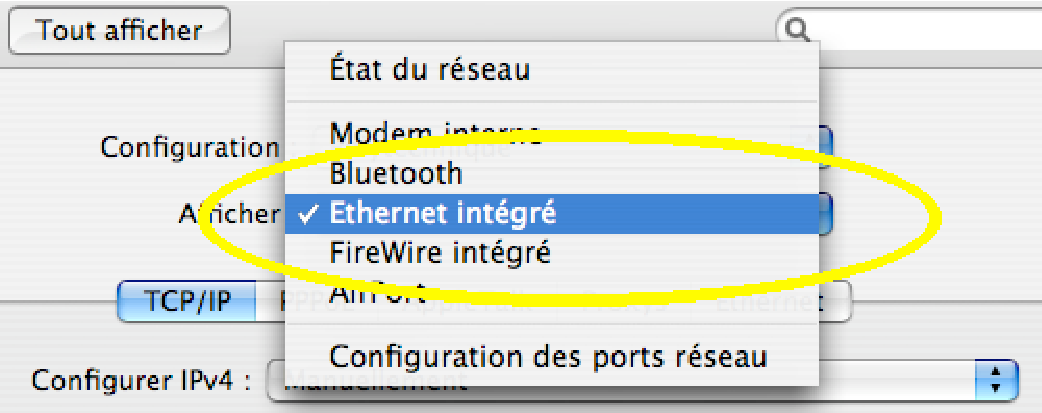
\includegraphics[width=0.96 \textwidth]{images/mac_config_ethernet}} \\ 
 		{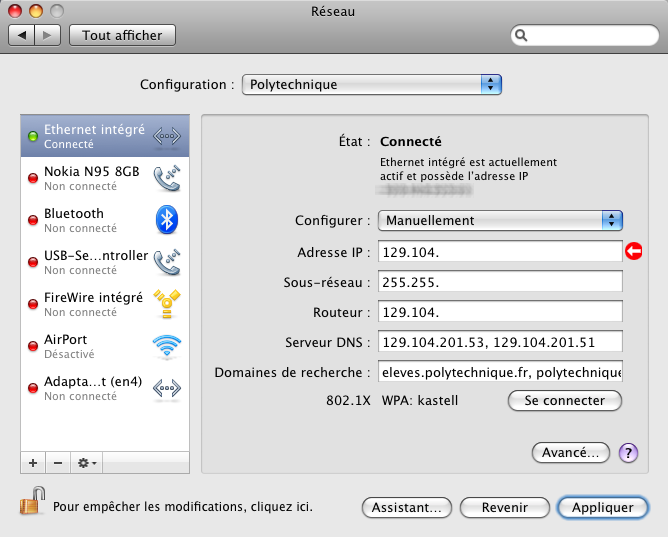
\includegraphics[width=0.96 \textwidth]{images/mac_config_ip_leopard}} \\
 		{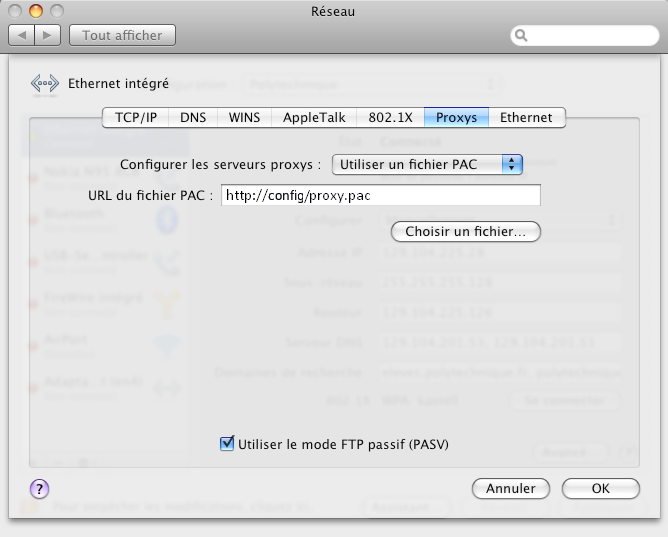
\includegraphics[width=0.96 \textwidth]{images/mac_config_proxy_leopard}}
\end{flushright}
 		\end{minipage}
 		 	\label{config:mac:ip:leopard}	}
     	 \caption{Cr\'eer une nouvelle configuration r\'eseau}

    \end{center}
  \end{figure*}

\pagebreak

La gestion des configurations r\'eseau de Mac OS X permet de cr\'eer plusieurs configurations et de passer en un clic de l'une  l'autre gr\^ace au sous-menu \menu{Configuration R\'eseau} du menu \menu{Pomme}. Cela est tr\`es pratique pour les machines vou\'ees \`a  \^etre connect\'ees \`a  plusieurs endroits successivement --- les portables par exemple (voir la page~\pageref{wifi} puis la section \emph{Wi-Fi} pour plus de pr\'ecisions sur le \emph{Wi-Fi}). Commence donc par cr\'eer une nouvelle configuration r\'eseau dans le menu d\'eroulant \menu{Configuration}.



Une fois la nouvelle configuration cr\'e\'ee, il faut configurer l'interface r\'eseau \emph{Ethernet}.



\app{Leopard} : Dans la colonne de gauche, s\'electionne \menu{Ethernet int\'egr\'e}.

Choisis alors \menu{Configurer IPv4} :% \menu{Manuellement} (\app{Tiger}) ou 
\menu{Configurer} : \menu{Manuellement} (\app{Leopard}). Tu trouveras toutes les valeurs d'adresses IP n\'ecessaires pour la configuration en page \pageref{calcul_ip} ou en te reportant aux captures d'\'ecran~\ref{config:mac:ip:leopard}. Si une partie d'adresse IP est blanche sur ces captures, c'est qu'elle t'est personnelle et que tu dois la calculer !


  
  

%\imageref{images/mac_config_ip_leopard}{0.4}{Configuration IP (Leopard)}{!ht}{config:mac:ip:leopard}}


Pour avoir acc\`es \`a  Internet, il faut aussi configurer le \emph{proxy}.

\app{Leopard} : Clique sur le bouton \menu{Avanc\'e...} puis sur l'onglet \menu{Proxys}.


\app{Mac OS X 10.3.3 et sup\'erieur} :  choisis l'option \menu{Configuration automatique de proxy} et indique http://config/proxy.pac comme URL de fichier PAC. Pour Mac OS X 10.3 \`a  10.3.2, n'oublie pas une fois que tu as le r\'eseau de faire la mise \`a  jour de ton syst\`eme, pour pouvoir configurer de fa\c con automatique le \emph{proxy}.

\app{Mac OS X 10.3.2 et inf\'erieur} : il te faut sp\'ecifier tous les
\emph{proxies} manuellement, et mettre \server{kuzh.polytechnique.fr}, port \server{8080}. Malheureusement, cele te permettra uniquement d'acc\'eder aux sites h\'eb\'erg\'es hors du plat\^al : les sites \'el\`eves ne fonctionneront pas.


N'oublie pas d'activer le mode passif pour les transferts en FTP, en cochant la case comme dans la capture.

\subsubsection{Configuration antivirus}

Bien qu'il soit important de maintenir ton syst\`eme \`a  jour, un antivirus est pour l'instant tout \`a  fait superflu sur Mac, puisqu'aucun virus fonctionnel n'a encore vu le jour. Attention cependant, n'ouvre pas des fichiers dont tu ne te sois pas assur\'e de la provenance, et essaie de te tenir au courant des actualit\'es concernant les failles des applications que tu utilises.

\subsubsection{Configuration web}
\flimage{images/nux_firefox_icon}{0.07}{l}
Un point particulier pour la configuration du \emph{proxy} de \app{Firefox} : dans \menu{Pr\'ef\'erences}, \menu{Avanc\'e}, \menu{R\'eseau}, clique sur \menu{Param\`etres} et, dans le champ \menu{Adresse de configuration automatique du proxy}, inscris : \urllink{http://config/proxy.pac}. 
\\
\\

\flimage{images/mac_safari_icone}{0.07}{l}
\app{Safari}, le navigateur web d'Apple, est maintenant compatible avec la majorit\'e des sites \emph{web}. Tu peux donc t'en servir au quotidien, en faisant appel \`a  \app{Firefox} pour les sites r\'ecalcitrants. Un conseil : pense \`a  activer le blocage des fen\^etres \emph{pop-up} (dans le menu \menu{Safari}). \app{Safari} peut aussi servir de client RSS (voir plus bas).\\
\\

\app{Google Chrome} se règle quant à lui automatiquement sur la configuration du système. 
\\

\subsubsection{Configuration \emph{mail}}
\flimage{images/mac_mail_icone}{0.07}{l} \app{Mail} : un client \emph{mail} offrant les fonctionnalit\'es classiques d'un bon client : recherche instantan\'ee, filtre antispam, r\`egles de tri automatique des \emph{mails}, regroupement des \emph{mails} correspondant \`a  une m\^eme discussion.

Au premier lancement, \app{Mail} te demandera de remplir les informations concernant ton compte \emph{mail} sur \server{poly}, il suffit de le remplir avec les donn\'ees suivantes :
\begin{description}
  \item[Nom complet] ton nom !
  \item[Adresse \'electronique] de la forme \mail{prenom.nom@polytechnique.edu}
  \item[Serveur de r\'eception] \server{poly.polytechnique.fr}
  \item[Type de compte] \menu{POP}
  \item[Nom d'utilisateur] ton \emph{login} \server{poly} (les huit premi\`eres lettres de ton nom en g\'en\'eral)
  \item[Mot de passe] ton mot de passe \server{poly}
  \item[Serveur d'envoi (SMTP)] \server{poly.polytechnique.fr} ou \server{ssl.polytechnique.org}
\end{description}

Si tu as d\'ej\`a  cr\'e\'e un compte pr\'ec\'edemment, il faut aller dans les \menu{Pr\'ef\'erences} (accessibles depuis le menu \menu{Mail}), onglet \menu{Comptes}, pour cr\'eer un autre compte en cliquant sur la case \menu{+}.

N'oublie pas de cocher \menu{Activer le cryptage SSL} dans l'onglet \menu{Avanc\'e}, port 995. Tu souhaiteras alors certainement installer le certificat de s\'ecurit\'e de \server{poly} (tu le trouveras sur \urllink{http://poly/}). Une fois que tu as t\'el\'echarg\'e le certificat, ouvre le fichier \menu{.CRT} obtenu, et dans \app{Trousseau d'acc\`es}, installe-le dans %\menu{X509Anchors} (Tiger) ou 
\menu{session} (Leopard).

Cette configuration marche pour acc\'eder \`a  ses mails depuis l'int\'erieur de l'X mais aussi de l'ext\'erieur, sans rien changer. En revanche tu ne peux pas envoyer de \emph{mails} depuis l'ext\'erieur , car le serveur \server{poly} ne le permet pas. Nous te conseillons vivement d'utiliser le serveur SMTP \server{polytechnique.org} et de regarder la configuration propos\'ee par \urllink{Polytechnique.org}. Celle-ci permet d'envoyer des \emph{mails} s\^urs \`a  l'ext\'erieur de l'\'Ecole sans modifier ta configuration par la suite. Tu peux ajouter ce SMTP dans l'onglet \menu{Comptes} des \menu{Pr\'ef\'erences} de \emph{mail} et r\'egler dans l'onglet \menu{Avanc\'es} comme dans la capture.

\begin{figure*}[!hl]
    \begin{center}
	      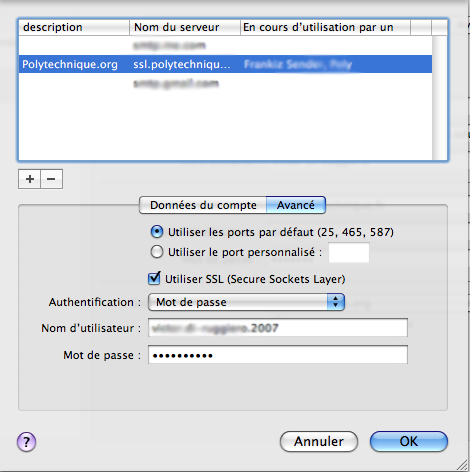
\includegraphics[width=0.4\textwidth]{images/mac_config_smtp_poltechnique.png} 
      \caption{Configurer le serveur SMTP \server{Polytechnique.org}}
    \end{center}
  \end{figure*}

Le LDAP ne fonctionne pas \`a  l'heure actuelle avec \app{Mail} (mars 2009) sous \app{Leopard}, contrairement aux  autres syst\`emes d'exploitation (fonctionne cependant avec \app{Thunderbird}).
%\subsuEnfin, tu peux disposer dans \app{Mail} de l'annuaire de l'\`acole, mis \`a  disposition par la DSI. Pour cela, va dans les \menu{Pr\'ef\'erences} de Mail,
%puis dans la rubrique \menu{R\'edaction} et clique sur \menu{Configurer LDAP\ldots}. Tu peux ensuite utiliser le bouton \menu{+} pour ajouter un
%serveur, et remplir la fen\^etre comme sur la capture.

%\imagepos{images/mac_config_ldap}{0.6}{Configurer l'annuaire}{!ht}
%bsection{Logiciels additionnels}

Les logiciels suivants sont utiles pour utiliser avec Mac OS X les services propos\'es sur le r\'eseau ; ils sont t\'el\'echargeables sur \server{frankiz}, dans la rubrique \menu{T\'el\'echarger}, \menu{Mac}.

%\subsubsection{Configuration \emph{news}}
%
%\flimage{images/mac_thunderbird_icone}{0.07}{l} 
%\app{Thunderbird} : un client \emph{news} permettant d'acc\'eder aux forums de discussion des \'el\`eves (voir page~\pageref{newsgroups} pour les d\'etails sur \server{frankiz}), mais aussi \`a  ceux de \server{usenet} gr\^ace au serveur \server{polynews.polytechnique.fr}. Il est tr\`es proche d'\app{Outlook Express} dans son esprit. Dans la m\^eme cat\'egorie, il existe \app{MacSOUP}, \app{Unison} ou encore \app{MT-NewsWatcher}. La configuration se fait de la m\^eme mani\`ere.
%
%Au premier lancement, l'application te propose d'importer les param\`etres depuis une autre application. Clique sur \menu{Suivant}. Tu peux alors choisir quel type de compte tu veux configurer (tu remarqueras que tu peux aussi cr\'eer un compte courrier \'electronique, et un compte RSS). S\'electionne \menu{Compte forums de discussion} et clique sur \menu{Suivant}. Entre alors les informations suivantes :
%
%\begin{description}
%  \item[Votre nom] ton nom ou ton pseudo
%  \item[Adresse de courrier] \mail{prenom.nom@polytechnique.edu}
%  \item[Serveur de forums] \server{news}
%  \item[Nom du compte] News Frankiz
%  \item[Nom d'utilisateur] ton \emph{login }poly (les huit premi\`eres lettres de ton nom en g\'en\'eral)
%  \item[Serveur d'envoi (SMTP)] \server{poly.polytechnique.fr} ou \server{ssl.polytechnique.org}
%\end{description}
%
%
%Pour t'abonner \`a  des groupes de discussion, il te suffit de s\'electionner le compte \menu{News Frankiz} dans la fen\^etre \menu{Dossiers} de \app{Thunderbird}, puis de cliquer sur \menu{G\'erer les abonnements aux groupes de discussion}. Tu pourras ensuite s\'electionner les forums qui t'int\'eressent parmi la liste propos\'ee. Reporte-toi \`a  la page \pageref{newsgroups} pour plus d'infos sur les \emph{newsgroups} auxquels t'abonner !
%

\subsubsection{Autres logiciels utiles}

%\flimage{images/mac_qrezix_icone}{0.07}{l} \app{qRezix} : en deux mots, c'est un programme d\'evelopp\'e par le BR pour faciliter la vie sur le r\'eseau. Tu peux le r\'ecup\'erer via le lien qRezix sur \server{Frankiz} ou sur \urllink{http://br.frankiz.net/qrezix/mac/}. Pour plus de d\'etails, voir le paragraphe consacr\'e \`a  qRezix \`a  la page \pageref{qrezix}. \\

%\app{Leopard} : le pare-feu se r\`egle pour chaque application; tu n'auras qu'\`a  r\'epondre \menu{Autoriser} lorsqu'il te demandera si tu veux \menu{Autoriser les connexions entrantes}.

%\noindent  \app{Tiger} : Attention, si ton \emph{firewall} est activ\'e, tu dois ouvrir les ports 5050, 5053 et 5055 en TCP. Pour cela va dans \app{Pr\'ef\'erences Syst\`eme}, dans le module \menu{S\'ecurit\'e}, onglet \menu{Coupe-feu}. S'il est \'ecrit \menu{Coupe-feu activ\'e}, clique le bouton \menu{Nouveau} et remplis la bo\^ite de dialogue comme sur la capture d'\'ecran ci-dessous pour ouvrir les ports.

%\imagepos{images/mac_firewall}{0.5}{Ouvrir les ports pour \app{qRezix} (Tiger)}{!ht}

%\flimage{images/mac_conversation_icone}{0.1}{l}
%\noindent\app{Colloquy}, un client IRC dans le m\^eme esprit qu'\app{iChat}. Il dispose d'une interface tr\`es simple ne n\'ecessitant pas de conna\^itre les commandes IRC. Tu peux te reporter \`a  la page \pageref{irc} pour plus d'infos sur l'IRC. \app{X-Chat Aqua} est un autre client IRC, plus riche en fonctionnalit\'es, mais moins agr\'eable \`a  utiliser. \\

%\flimage{images/mac_netnewswire_icone}{0.1}{l}
%\noindent\app{NetNewsWire} est la r\'ef\'erence des clients RSS sur Mac, et est maintenant gratuit. Dans le m\^eme genre, on peut citer \app{Vienna}, un client RSS open source, dont le d\'eveloppement actif est prometteur. Les flux RSS permettent d'agr\'eger dans un seul logiciel des informations en provenance de nombreux sites web, qui peuvent provenir de forums de discussions, de mises \`a  jour de logiciels, d'informations internationales\dots \\ \\

%\flimage{images/mac_fink_icone}{0.07}{l} \app{Fink} est la mani\`ere la plus simple d'installer sur Mac OS X nombre de logiciels issus du monde Unix (Linux par exemple). Gr\^ace \`a  lui, tu pourras installer les m\^emes logiciels que dans les salles informatiques. Par exemple, tu pourras installer Scilab sans trop de peine\dots La configuration n\'ecessaire se trouve sur la page \urllink{http://frankiz/binets/reseau/Miroir\_Fink}.\\ 

\flimage{images/logo_Windows}{0.1}{l}
 \app{Windows et les Mac Intel} : Maintenant il est possible d'installer Windows gr\^ace \`a  \app{Boot Camp}, livr\'e avec \app{Leopard}. Cela te permettra de profiter des quelques applications du monde PC qui valent le coup tout en gardant ton Mac. Tu peux \'egalement virtualiser Windows (utiliser Windows en utilisant en m\^eme temps Mac OS) gr\^ace \`a  \app{VMware Fusion}, \app{VirtualBox} ou \app{Parallels Desktop}. Le  d\'efaut de cette solution est que tu n'as pas d'acc\'el\'eration 3D, donc pour les jeux il te faudra red\'emarrer. Ces trois logiciels sont disponibles sur leurs sites \emph{web} respectifs. \`A toi de choisir !
Mais v\'erifie tout de m\^eme que tu as bien un processeur Intel (\menu{Pomme} puis s\'electionne \menu{\`A propos de ce Mac}).

\clearpage


\markright{Pour bien commencer}
\subsection{\emph{Wi-Fi}}
La DSI propose actuellement un réseau \emph{Wi-Fi}, qui couvre le grand hall, les amphis, les salles de PC, le bataclan (bâtiment qui va de la Kès au bâtiment des
binets/langues), le bâtiment des binets/langues.

Pour te connecter au \emph{Wi-Fi} avec Windows, Mac, Linux ou un iPhone, tu trouveras les instructions sur la page \urllink{http://wifi}.

Avec Windows, \textbf{avant Windows 8}, tu dois téléchager un logiciel appelé \app{SecureW2} qui est fourni par la DSI sur son site, \urllink{http://www.dsi.polytechnique.fr/fr/telecommunications/wifi/}. Ce n'est plus nécessaire depuis Windows 8.

Avec Mac OS X Lion ou iOS (iPhone, iPad), il faut télécharger un fichier 
\newline \file{Ecole-Polytechnique.mobileconfig} dont le lien se trouve sur \urllink{http://wifi}. Pour des versions plus anciennes de Mac OS, consulte \urllink{http://br.binets.fr/Configuration\_du\_WiFi\_sous\_Mac}. Attention, avec iOS7, il arrive que le fichier .mobileconfig fourni par la DSI ne marche pas, tu peux essayer avec celui là: \urllink{br.binets.fr/files/WifiPoly.mobileconfig}.

Avec Linux ou Android, les noms des paramètres dépendent du système utilisé, mais voici un tableau récapitulatif :
\begin{center}
\begin{tabular}{r|l}
 SSID & Polytechnique \\
 Nom d'utilisateur/Mot de passe & Identifiants DSI (salle info) \\
 Sécurité & WPA1 Entreprise \\
 Gestion des clés & WPA-EAP \\
 Pairwise & TKIP \\
 Authentification & Tunneled TLS (TTLS) ou EAP-FAST \\
 Authentification interne & PAP \\
 Proxy HTTP pour tous les protocoles & 129.104.247.2 (port 8080) \\
 Serveurs DNS & 129.104.201.53, 129.104.201.51
\end{tabular}
\end{center}




%Deux réseaux ont été déployés :

%\begin{description}
%  \item[keriadenn] : c'est le réseau public, qui te permet uniquement d'accéder au portail wifi (\url{http://wifi/}, accessible également depuis le réseau normal). Tu trouveras à cette adresse toutes les informations de configuration nécessaires pour te connecter au second réseau, \server{kastell}.

%  \item[kastell] : réseau protégé et caché qui permet, après authentification, de te connecter au réseau et à Internet comme si tu étais dans ton casert !
%\end{description}


\subsection{Acc\`es aux ordis des salles infos depuis chez toi}

                 
  \paragraph{WinSCP} Un logiciel pratique qui te permet de te connecter en salle info.
                  Son fonctionnement est expliqu\'e en d\'etails dans le WikiX (\urllink{http://winscp.net}).  \\
                  Voir aussi \app{Putty} (\urllink{http://www.putty.org/}).

